\section{Project Usecase Diagram}
\begin{figure}[H]
    \centering
    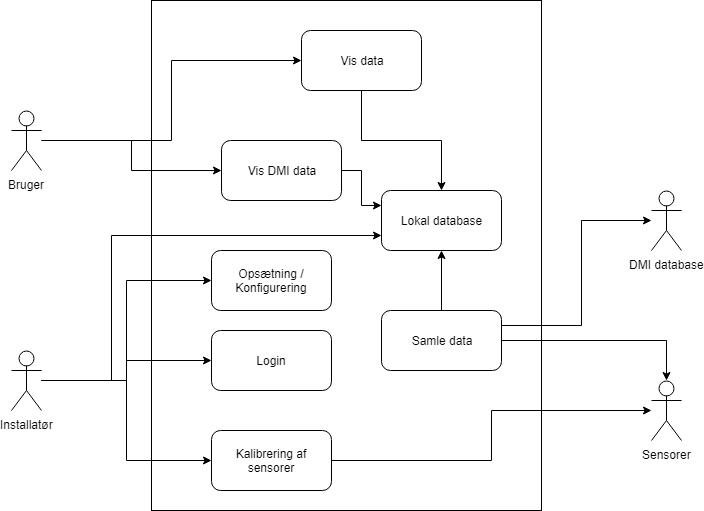
\includegraphics[width=0.8\linewidth, height=8.5cm]{Struktureret_System_Udvikling/Workshop_1/Assets/IoT_weather_station.png}
    \caption{Usecase Diagram}
    \label{fig:my_label}
\end{figure}
Systemet indeholder som usecase diagrammet anviser fire forskellige aktører:\\
En bruger, der kan få vist den indsamlede data, gennem en af de to mulige grænseflader, for henholdsvis den samlede Sensor data, eller den lokale udsigt opdateret fra DMI.\\
En installatør, der gennem en netbaseret forbindelse kan loggein i systemet, for efterfølgende at administrere produktet, ved f.eks. opsætning eller omkonfigurering, sensor kalibrering, eller datamanipulation.\\
En række sensorer der bidrager med forskellige målte data til systemets lokale information, som senere kan fremvises til brugeren.\\
Og en tilgang til DMI's kommende vejrudsigt, der bliver opdateret for brugerens oplevelse.
\\\\
\noindent
Produktets tænkte leveprocess tænkes som:\\
Brugeren køber produktet fra en producent eller distributør.\\
Installerer produktet i sit hjem ved hjælp af den medfølgende manual, og op-kobler produktets hovedmodul til en lokal netværksruter.\\
Efterfølgende kan brugeren tilgå hovedmodulet gennem dens uddelte lokale ipaddresse, fra f.eks. en lokal computer.\\
Igennem denne forbindelse til hovedmodulets, vil brugeren blive guidet gennem en førstegangs opsætnings wizzard.\\
Her efter kan denne forbindelse også bestyres eller konfigurere gennem denne samme tilgang.
Hvis enkelte sensorer skulle blive beskadiget, kan enkelte sensorer købes fra producenten.
Et produkt kan altid manuelt gensættes til fabriks indstillinger.